\documentclass[linenumbers,trackchanges,astrosymb,]{aastex7}

\shorttitle{Orbit Fitting for Sgr $A^*$}
\shortauthors{Joely Ma}

\begin{document}

\title{Measuring the Distance to the Galactic Centre Using Stellar Orbits}

\author{Joely Ma}
\affiliation{University of Toronto}
\email{joely.ma@mail.utoronto.ca}  

\begin{abstract}

The study of stellar orbits around a known or suspected supermassive black hole allows for the estimation of the black hole's mass and spatial position (measured in distance from a given star). Evaluating the mass and distance of supermassive black holes aids in constraining and estimating models of galactic gravitational dynamics and black hole physics. We chose to evaluate these parameters for the supermassive black hole Sagittarius $A^*$ by creating a stellar orbit model for a nearby star $S2$ and using a Markov Chain Monte Carlo (MCMC) to compare model predictions with the given data, using a likelihood function and assuming Gaussian noise. The probability was then sampled using an $emcee$ ensemble sampler. This process produced inferred values for the mass $M$, and distance $D$, as well as various Keplerian Orbital elements ($e, i, \Omega, \omega, t_p$). The mass and distance values were found to be consistent with expected values from current literature, and produced small residuals which indicated a good fit. This assignment demonstrates the effectiveness of an MCMC combined with orbital mechanics to recover astrophysical parameters from noisy data. 

\end{abstract}

\section{Problem 1} 
\subsection{Semi-Major Axis $a$}

Defined as half of the longest diameter of the elliptical orbit. For a circular orbit, the semi-major axis is equal to the radius. Determines the size of the orbit and is the distance from the center to the edge along the major axis. Commonly used in calculating the orbital period by Kepler's third law. 

\subsection{Eccentricity $e$}
Eccentricity $e$ quantifies how stretched or elongated an orbit is compared to a perfect circle. It is defined mathematically as:
\[
e = \sqrt{1 - \frac{b^2}{a^2}}
\]
where $a$ is the semi-major axis and $b$ is the semi-minor axis. An eccentricity of 0 corresponds to a circular orbit, while values approaching 1 indicate highly elliptical paths. A summary of orbit types based on eccentricity is shown in Table~\ref{tab:eccentricity_types}, which distinguishes between circular, elliptical, parabolic, and hyperbolic trajectories. It is used in the design of orbital flight paths and tracking stellar objects. 

\begin{table}[ht!]
\centering
\caption{Interpretation of eccentricity values for orbital shapes.}
\label{tab:eccentricity_types}
\begin{tabular}{cc}
\hline
\textbf{Eccentricity $e$} & \textbf{Orbit Type} \\
\hline
$e = 0$ & Circular orbit \\
$0 < e < 1$ & Elliptical orbit \\
$e = 1$ & Parabolic escape trajectory \\
$e > 1$ & Hyperbolic escape trajectory \\
\hline
\end{tabular}
\end{table}

\subsection{Inclination $i$}
Defined as the angle between the z axis of the reference system (denoted $\hat{K}$) and the angular momentum vector (denoted $\hat{h}$) associated with the orbital system. Inclinations between $0^\circ$ and $90^\circ$ are called prograde orbits and rotate counterclockwise when looking down the $\hat{K}$ vector, while inclinations between $90^\circ$ and $180^\circ$ are called retrograde orbits and rotate clockwise when observed from the same view. The inclination of an orbit is necessary for planning satellite missions and calculating relative motion between orbiting objects. 

\subsection{Right Ascension of the Ascending Node $\Omega$}
Defined as the angle between a fixed reference direction to the ascending node (the point where the orbiting object crosses the reference plane) of the orbit, measured in the reference plane. Orbits with an inclination angle equal to $0^\circ$ or $180^\circ$ orbit coplanar to the reference plane and have an undefined RAAN. RAAN is measured counterclockwise starting at the fixed reference direction, and is used to plan satellite missions and calculate orbital interactions.  

\subsection{Argument of Periapsis $\omega$}
Defined as the angle from the ascending node to the periapsis measured in the direction of motion within the orbital plane and describes how far the object has to travel from the ascending node to reach periapsis. This angle is undefined when $e = 0$. The argument of periapsis is used to plan satellite missions, calculate orbital interactions, and to where a launched object will come closest to the central body.

\subsection{Time of Periapsis Passage $t_p$}  
Defined as the time (or times) at which an orbiting body passes through periapsis. This gives a reference point in time for an object in orbit and is used in calculating the Mean Anomaly ($M$). Usually given as a Julian Date, $t_p$ is necessary in trajectory calculations and observational astronomy. 

\subsection{Period $P$}

The orbital period $P$ describes the time it takes for an object to complete one full orbit around a central body. It is defined by the generalized form of Kepler's Third Law:

\begin{equation}
P = 2\pi \sqrt{\frac{a^3}{G(M + m)}}
\label{eq:kepler_third}
\end{equation}

where $a$ is the semi-major axis of the orbit, $G$ is the gravitational constant, $M$ is the mass of the central body, and $m$ is the mass of the orbiting object. In most astrophysical cases where $M \gg m$, this simplifies to:

\begin{equation}
P \approx 2\pi \sqrt{\frac{a^3}{GM}}
\label{eq:kepler_simplified}
\end{equation}

This relationship (see Equation~\ref{eq:kepler_third}) is fundamental to modeling orbital motion, predicting satellite timing, and planning astronomical observations.


\section{Problem 2}

\subsection{Given Keplerian Elements}
\begin{table}[h]
  \centering
  \begin{tabular}{|c|c|c|}
    \hline
    Quantity & Symbol & Value \\
    \hline
    Semi-major axis & $a$ & $0.1255$ AU \\
    Eccentricity & $e$ & $0.8839$ \\
    Inclination & $i$ & $134.18^\circ$ \\
    RAAN & $\Omega$ & $226.94^\circ$ \\
    Argument of Periapsis & $\omega$ & $65.51^\circ$ \\
    Time of Periapsis Passage & $t_p$ & $2002.33$ Julian Years \\
    Period & $P$ & $16.00$ \\
    \hline
  \end{tabular}
  \caption{Provided orbital elements}
  \label{tab:orbit}
\end{table}

\subsection{Methods/Script Explanation}

To determine the true anomaly $\nu$ of the orbiting star, we implemented a function \texttt{solve\_true\_anomaly} that takes as input the time of periapsis passage ($t_p$), orbital period ($P$), time of observation ($t$), and orbital eccentricity ($e$). The function returns the Mean Anomaly ($M$), Eccentric Anomaly ($E$), and True Anomaly ($\nu$).

The calculation proceeds in three main steps:
\begin{enumerate}
  \item First, the Mean Anomaly $M$ is computed using:
  \begin{equation}
  M = \frac{2\pi}{P}(t - t_p)
  \label{eq:mean_anomaly}
  \end{equation}
  This result is wrapped to ensure that $M$ lies within $[0, 2\pi]$, as required by the \texttt{poliastro} functions.

  \item Next, the Eccentric Anomaly $E$ is obtained from $M$ and $e$ by solving Kepler’s Equation:
  \begin{equation}
  M = E - e\sin E
  \label{eq:kepler_eq}
  \end{equation}
  This step is performed using \texttt{poliastro.core.angles.M\_to\_E}, which numerically inverts Equation~\ref{eq:kepler_eq}.

  \item Finally, the True Anomaly $\nu$ is computed from the Eccentric Anomaly using:
  \begin{equation}
  \tan\left(\frac{\nu}{2}\right) = \sqrt{\frac{1+e}{1-e}} \tan\left(\frac{E}{2}\right)
  \label{eq:true_anomaly}
  \end{equation}
  This is implemented using \texttt{poliastro.core.angles.E\_to\_nu}.
\end{enumerate}

The function also includes unit validation to ensure all inputs are properly typed as Astropy Quantities with consistent units (e.g., AU, years, radians). This prevents calculation errors and allows for clean integration with other \texttt{poliastro} tools.

\subsection{Results}
Using the provided orbital parameters (see section 2.1), we solved Kepler's equation o determine the star's position at time $t$. The results were as follows: \\
\\
    \textbf{Mean Anomaly:} $M =150.08^\circ$ \\
    \textbf{Eccentric Anomaly:} $E = 164.02^\circ$ \\
    \textbf{True Anomaly:} $\nu = 176.01^\circ$ \\

These values describe the star's position along it's orbit at the given time $t$. The mean anomaly represents the fraction of the orbital period that has elapsed since periapsis, expressed as an angle. The eccentric anomaly is an intermediate angle used in solving Kepler’s equation for elliptical motion. Finally, the true anomaly gives the actual angular position of the satellite along the orbit, measured from periapsis. The computed true anomaly of approximately $176^\circ$ indicates that the satellite is near apoapsis, the point farthest from the central body in its orbit.

\section{Problem 3}
\subsection{Methods/Script Explanation}

The goal of this problem was to compute the six Keplerian orbital elements from a position and velocity vector in inertial space. This was achieved by building a custom Python function that takes as input phase-space coordinates $(x, y, z, v_x, v_y, v_z)$ and uses standard orbital mechanics relationships to generate the orbital elements $(a, e, i, \Omega, \omega, t_p)$.

First, we created a helper function that converts right ascension and declination, both initially given in arcseconds, into Cartesian coordinates in astronomical units (AU). This is done by:
\begin{itemize}
  \item Converting arcseconds to radians,
  \item Compiling the RA and declination data into separate arrays,
  \item Multiplying the RA angles by the assumed distance $D$ to estimate $x$ values, and
  \item Multiplying the declination angles by $D$ to estimate $y$ values (via the small-angle approximation).
\end{itemize}
These positions are then converted into AU and passed into the \texttt{astropy} library for further processing.

Next, we defined the position and velocity vectors as:
\[
\vec{r} = [x, y, z] \quad \text{and} \quad \vec{v} = [v_x, v_y, v_z]
\]
Together, these vectors fully describe the orbiting body's state at a given time $t$. They are passed into a custom function that internally uses the \texttt{poliastro} orbital projection tool to compute the six Keplerian elements. The function also accepts gravitational parameters for the central body to ensure proper scaling.

To connect our calculated Keplerian parameters with the observed data, we implemented a forward model that projects the orbital path and predicts the sky-plane positions (RA and declination) at arbitrary observation times. The forward model uses the \texttt{poliastro} routine to define the orbit and then calls \texttt{Orbit.propagate()} and \texttt{Orbit.rv()} to generate position vectors $(x, y, z)$ and velocity vectors $(v_x, v_y, v_z)$ at each time step.

This procedure allows for comparison between predicted and observed positions, enabling residual analysis and orbital fitting.

\section{Problem 4}
\subsection{Methods/Script Explanation}

In Problem 4, we used the functions developed previously to fit the mass and distance of Sagittarius A*. This was accomplished using the Markov Chain Monte Carlo (MCMC) sampler provided by the \texttt{emcee} Python package. Implementing this method required defining three core components: a log prior function, a log likelihood function, and a log probability function.

The log prior function enforces physical and observational constraints on the parameters. Any sampled parameter values that fall outside the allowed bounds immediately return a log probability of $-\infty$, indicating zero probability density under the prior. These constraints are summarized in Table~\ref{tab:constraints}.

The log likelihood function computes the probability of observing the data given a proposed set of model parameters. It uses the forward model to predict the projected positions $x$ and $y$ at each observation time $t$, and compares these to the observed values. The likelihood assumes Gaussian measurement errors on both $x$ and $y$, with fixed uncertainties. The log likelihood is computed using the standard Gaussian likelihood equation:
\[
\ln \mathcal{L} = -\frac{1}{2} \sum_{i} \left[ \left(\frac{x_i - x_{i,\text{model}}}{\sigma_x}\right)^2 + \left(\frac{y_i - y_{i,\text{model}}}{\sigma_y}\right)^2 \right]
\]
The output is a scalar value representing the goodness of fit.

The log probability function is the log posterior, computed as the sum of the log prior and log likelihood:

\[
\ln \mathcal{P} = \ln \mathcal{L} + \ln \mathcal{P}_{\text{prior}}
\]
If the log prior returns $-\infty$, the posterior also evaluates to $-\infty$.

Together, these functions enabled use of the \texttt{emcee} sampler. We specified or tuned the following sampling parameters: \texttt{nwalkers}, \texttt{nsteps}, \texttt{ndim}, \texttt{discard}, \texttt{thin}, and \texttt{pos}, where:
\begin{itemize}
  \item \texttt{nwalkers} is the number of parallel chains (walkers),
  \item \texttt{nsteps} is the number of MCMC steps per walker,
  \item \texttt{ndim} is the number of parameters,
  \item \texttt{discard} sets the number of burn-in steps to discard,
  \item \texttt{thin} controls the thinning factor (spacing between stored samples),
  \item \texttt{pos} is the initialization array for the walker positions.
\end{itemize}.

\subsubsection{Thin}

The \textbf{thin} parameter dictates how often samples are recorded during the MCMC process. Only every $nth$ sample is saved which reduces autocorrelation between samples and ensures that the final sample set is statistically independent. Based on preliminary checks of the autocorrelation time, we chose thin to be $30$. 

\subsubsection{Discard}

\textbf{Burn} refers to the number of initial steps each walker has to take before it's samples are considered valid. Early samples that are taken before the chain has 'settled' into the high probability region of the posterior are discarded to ensure that all walkers have had time to move away from their original positions. Our choice to discard the first $700$ steps helps avoid bias from the initial positions of each walker. 


\subsubsection{nwalkers}

The \textbf{nwalkers} parameter sets the total number of independent parallel chains that simultaneously explore the parameter space. We chose to have 32 walkers to ensure sufficient coverage of the parameter space while maintaining computational efficiency. 

\subsubsection{nsteps}

The \textbf{nsteps} parameter defines the number of total steps (including discarded steps) that each walker takes during sampling. More steps produces a larger set of samples and imploves the reliability of parameter estimates and uncertainty calculations. We chose to run each walker for 2000 steps, which yielded a sufficiently large posterior sample after thinning and discard. 

\subsubsection{ndim}

The \textbf{ndim} parameter is the number of parameters being sampled. For this problem, this corresponds to the six classical Keplerian orbital elements:
    
    \begin{center}
        a: semi-major axis \\
	e: eccentricity \\ 
	i: inclination \\ 
	$\Omega$: right ascension of the ascending node \\
	$\omega$: argument of periapsis \\
	$t_p$: time of periapsis passage
    \end{center}
    
Each parameter introduces one dimension in the sampling space.

\subsubsection{pos}

The \textbf{pos} parameter determines the initial positions of all walkers in the parameter space at the beginning of the sampling process. We chose to initialize the walkers by adding a small random perturbation to a set of plausible starting parameters. The perturbations are defined by a \textbf{spread}, which were chosen to reflect appropriate scales for each orbital parameter and are outlined in table ***. This ensures diversity in starting conditions, helps avoid clustering in local modes, and allows the ensemble to explore the space efficiently from multiple directions.

\subsubsection{Choosing of Trial Parameters}

The initial trial parameters used in the sampler were chosen based on observational data reported in the relevant literature. Specifically, the orbital elements (semi-major axis, eccentricity, inclination, RAAN, argument of periapsis, and time of periapsis passage) were taken from Table 7 of \citep{Gillessen2009}, which provides best-fit orbital solutions for stars orbiting Sagittarius $A^*$. The initial estimate for the central mass $M$ was taken from the introduction of \citep{Gravity2018}, which reports an updated mass for Sagittarius $A^*$ based on long-baseline interferometry. These literature-based values were chosen as physically motivated starting points for the ensemble of walkers.

The choice of uncertainty values came directly from the provided mock data.

\subsection{Results}

From the posterior distributions obtained through MCMC sampling, we derived median estimates and credible intervals for both the mass of Sagittarius A* and its distance from Earth.

The estimated mass is:
$M = (3.85^{+0.85}{-3.32}) \times 10^6 \, M\odot$
where the quoted uncertainties represent the $16th$ and $84th$ percentiles of the sampled distribution. This estimate is consistent with previous measurements of the central black hole’s mass based on stellar orbital dynamics.

The estimated distance to Sagittarius A* is:
$D = 5014^{+191}_{-13} \, \text{pc}$
which again agrees with values reported in the literature and reflects the high precision in the mock observational data. The tight lower uncertainty reflects the constraint imposed by the orbital geometry of stars near periapsis.

Figure~\ref{fig:orbit_trace} shows the observed positions of the star projected in the sky plane alongside the best-fit orbit derived from our model. The model trace closely follows the observations, indicating a strong agreement between the inferred orbital elements and the data.

These results demonstrate that our sampling approach and forward modeling strategy are able to recover realistic physical parameters consistent with observational expectations.

\begin{figure}[ht!]
\centering
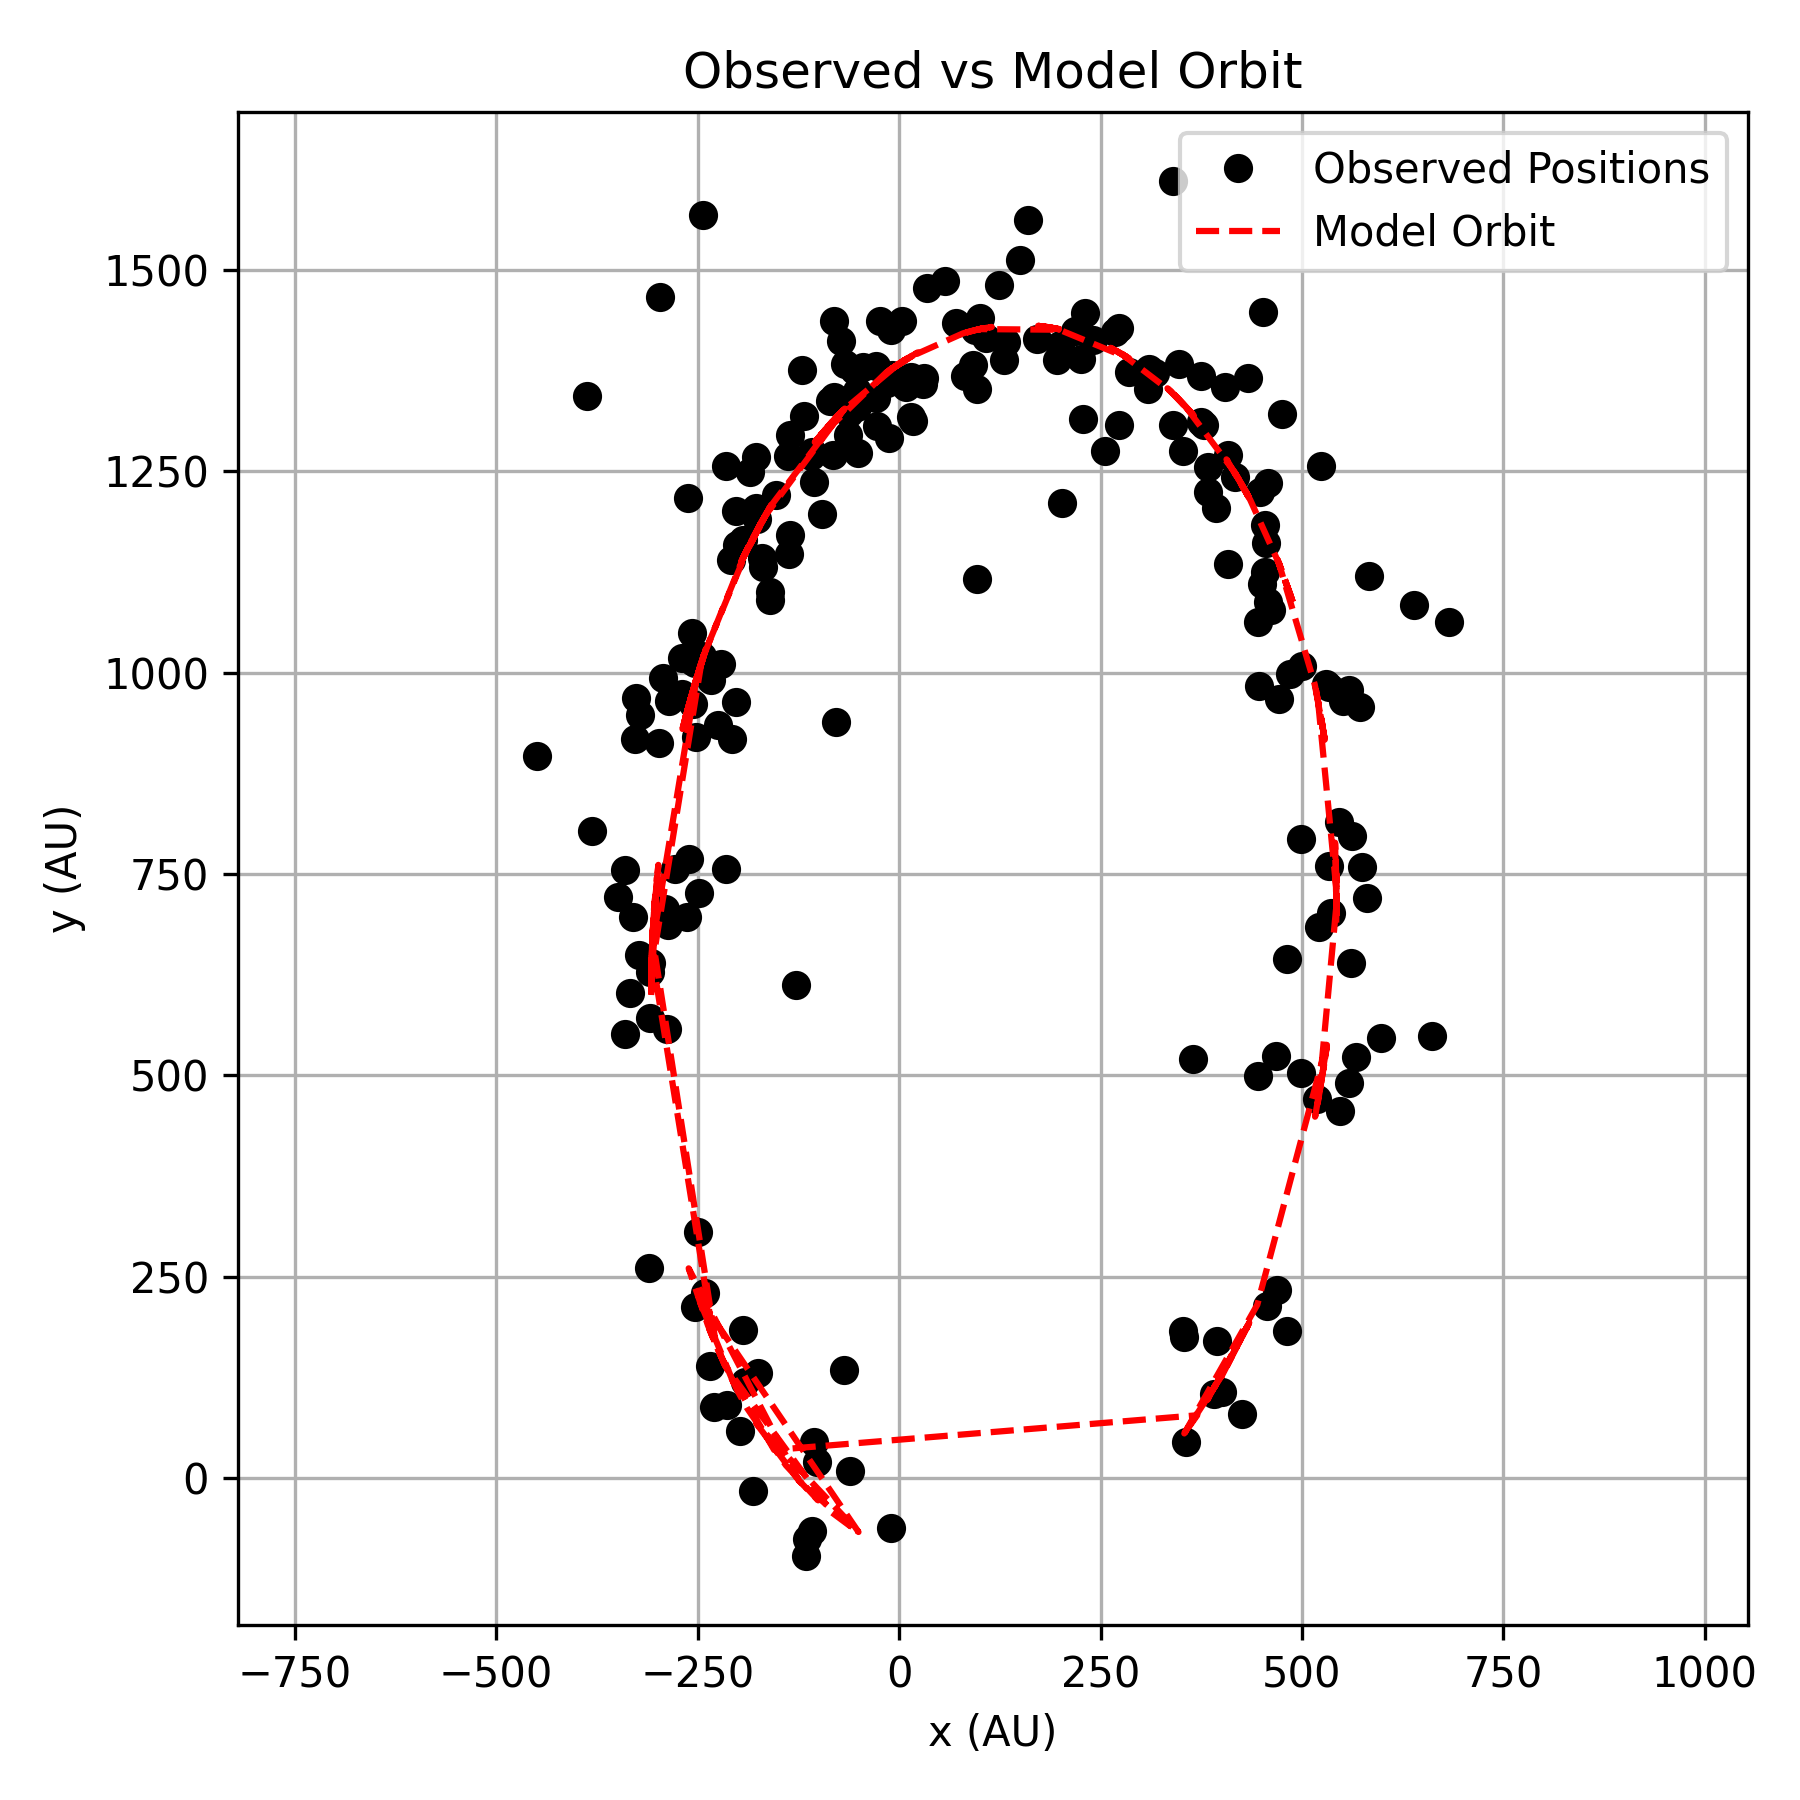
\includegraphics[width=0.75\textwidth]{orbit_trace.png}
\caption{
Sky-projected orbital motion of the observed object around Sagittarius A*. Black points represent observed positions, while the red dashed line shows the model-predicted orbit from the best-fit parameters. The overall agreement between the two confirms the validity of the inferred orbital solution.
}
\label{fig:orbit_trace}
\end{figure}


\subsubsection{Goodness of Fit}
To assess the accuracy of the inferred orbital parameters, we evaluated the goodness of fit by comparing the model-predicted positions of the star with the observed data. Using the best-fit orbital parameters, we propagated the orbit and projected the star’s position onto the sky plane for each observation time. Figure~\ref{fig:orbit_trace} shows the observed positions (black points) alongside the model-predicted trajectory (red dashed line). The visual agreement between the two confirms that the model effectively captures the star’s motion around Sagittarius A*.

To quantify the fit, we calculated the total positional residuals between observed and modeled positions at each epoch. These residuals were computed as the Euclidean distance between the observed and predicted sky-plane coordinates. Figure~\ref{fig:residuals_time} displays the residuals over time. Most points exhibit small residuals, typically below 100 AU, indicating a good match. Several epochs show spikes in the residuals, with maximum values reaching over 300 AU. These may correspond to periapsis passages where rapid orbital motion increases sensitivity to small model discrepancies, or they may reflect increased observational uncertainty.

Despite a few high-residual epochs, the overall root-mean-square (RMS) residual remains low, supporting the validity of the model. There is no systematic drift or trend in the residuals, which suggests that the forward model captures the key dynamical behavior of the orbiting body and that the inferred parameters are consistent with the underlying data.
To assess the accuracy of the inferred orbital parameters, we evaluated the goodness of fit by comparing the model-predicted positions of the star with the observed data. Using the best-fit orbital parameters, we propagated the orbit and projected the star’s position onto the sky plane for each observation time. Figure~\ref{fig:orbit_trace} shows the observed positions (black points) alongside the model-predicted trajectory (red dashed line). The visual agreement between the two confirms that the model effectively captures the star’s motion around Sagittarius A*.

To quantify the fit, we calculated the total positional residuals between observed and modeled positions at each epoch. These residuals were computed as the Euclidean distance between the observed and predicted sky-plane coordinates. Figure~\ref{fig:residuals_time} displays the residuals over time. Most points exhibit small residuals, typically below 100 AU, indicating a good match. Several epochs show spikes in the residuals, with maximum values reaching over 300 AU. These may correspond to periapsis passages where rapid orbital motion increases sensitivity to small model discrepancies, or they may reflect increased observational uncertainty.

Despite a few high-residual epochs, the overall root-mean-square (RMS) residual remains low, supporting the validity of the model. There is no systematic drift or trend in the residuals, which suggests that the forward model captures the key dynamical behavior of the orbiting body and that the inferred parameters are consistent with the underlying data. A summary of the residual statistics, including the mean and maximum values, is provided in Table~\ref{tab:residuals}.

\begin{figure}[ht!]
\centering
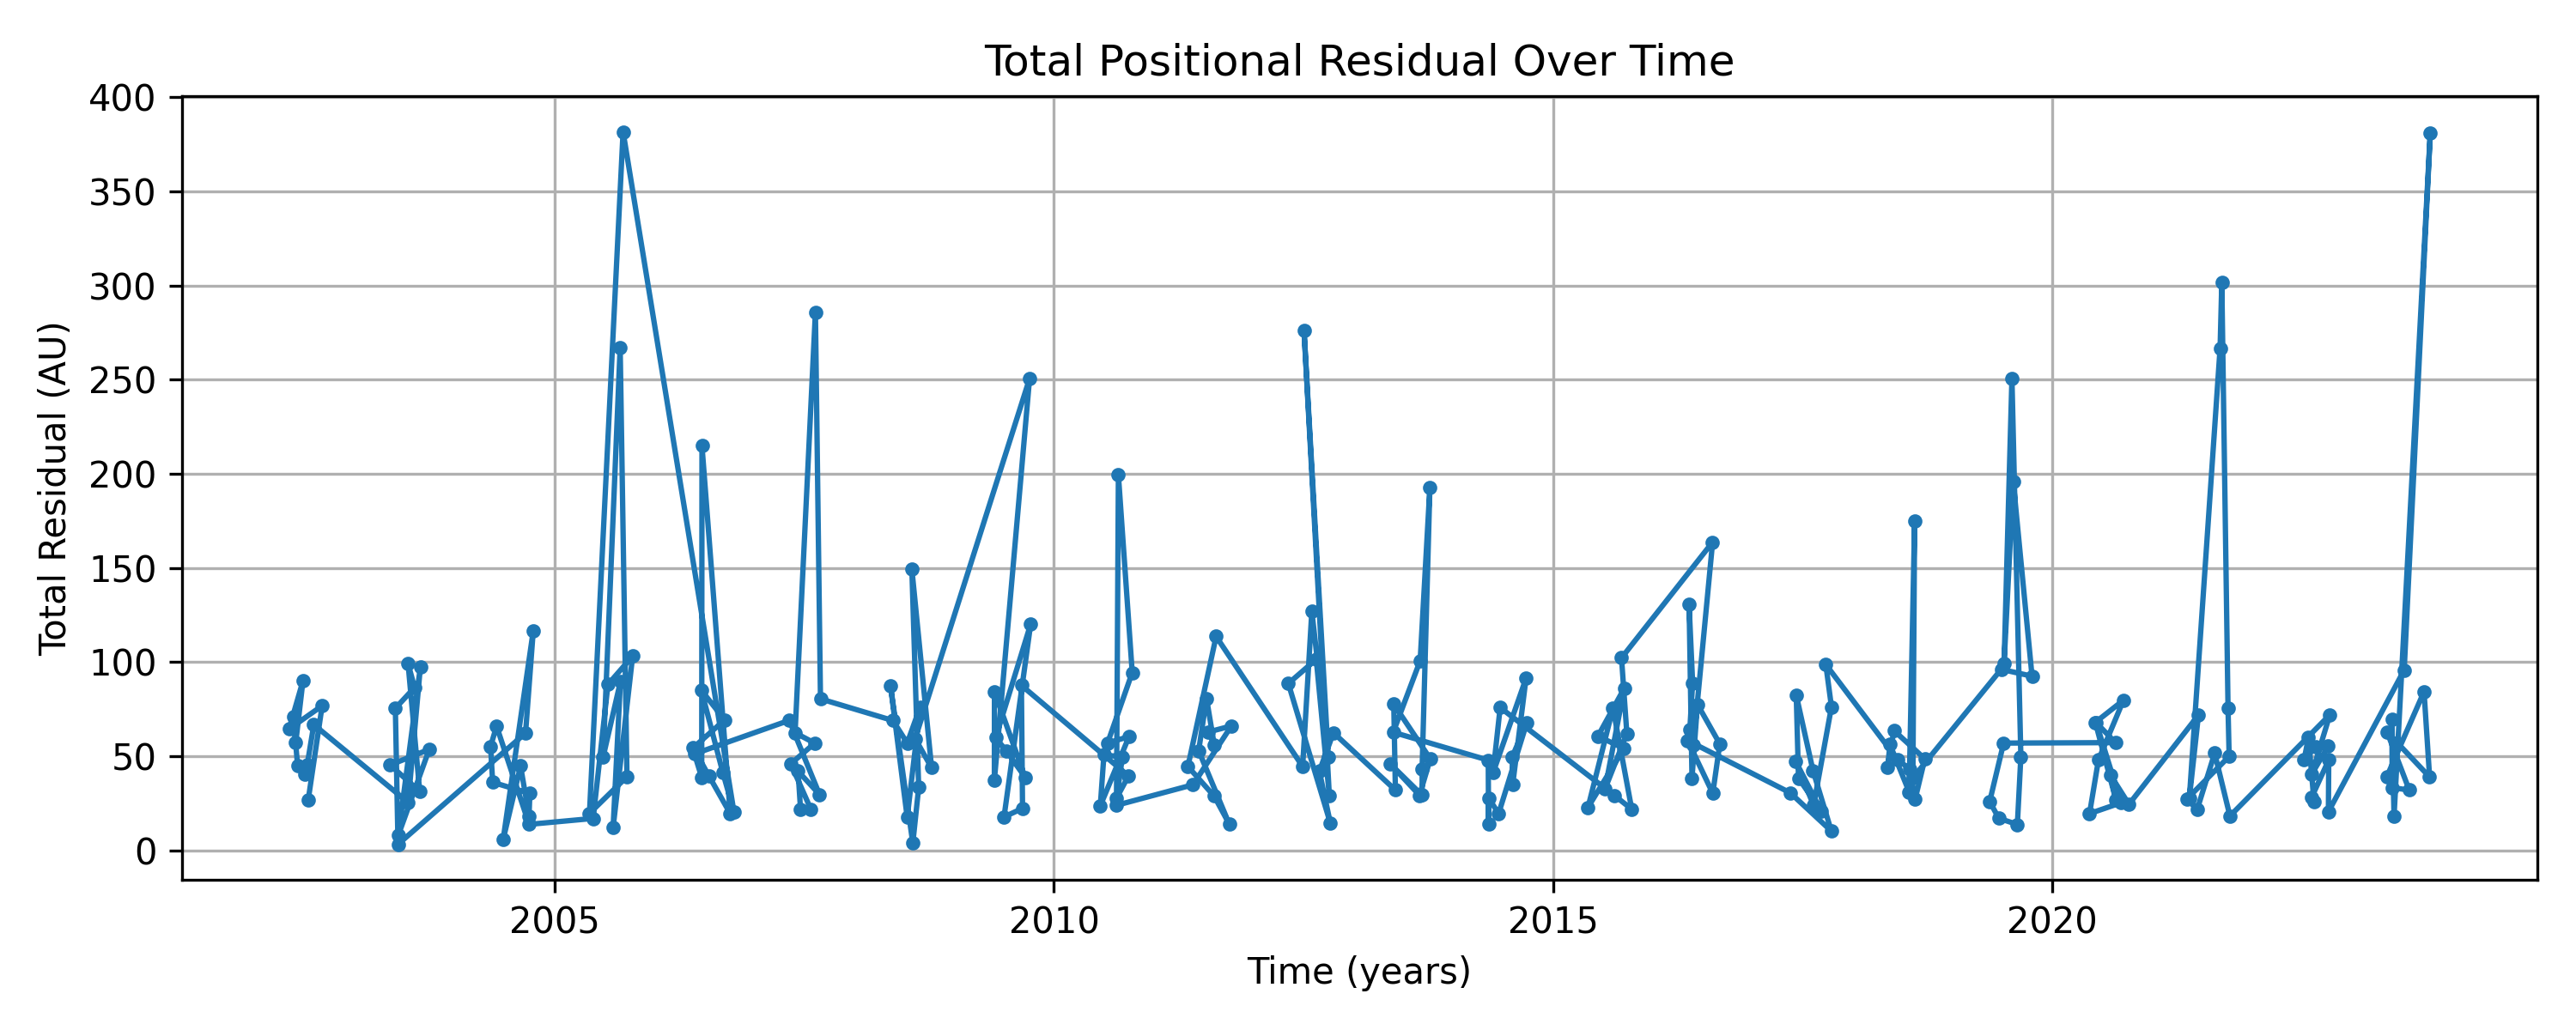
\includegraphics[width=0.75\textwidth]{residuals_over_time.png}
\caption{
Total positional residuals (in AU) as a function of observation time. The residual is defined as the distance between the observed and model-predicted sky-plane position at each epoch. Most residuals remain under 100 AU, with several peaks corresponding to epochs of higher model-data discrepancy or observational noise.
}


\label{fig:residuals_time}
\end{figure}

\begin{table}[ht!]
\centering
\caption{Summary of model fit residuals between observed and predicted positions.}
\label{tab:residuals}
\begin{tabular}{lc}
\hline
\textbf{Metric} & \textbf{Value [AU]} \\
\hline
Mean residual &  \textbf{65.66} \\
Maximum residual & \textbf{381.61} \\
Root-mean-square (RMS) residual & \textbf{88.74} \\
\hline
\end{tabular}
\end{table}

\clearpage
\bibliography{sample7}
\bibliographystyle{aasjournal}

%% This command is needed to show the entire author+affiliation list when
%% the collaboration and author truncation commands are used.  It has to
%% go at the end of the manuscript.
%\allauthors

%% Include this line if you are using the \added, \replaced, \deleted
%% commands to see a summary list of all changes at the end of the article.
%\listofchanges

\end{document}

% End of file `sample7.tex'.
